\documentclass[11pt]{article}            % Report class in 11 points
\parindent0pt  \parskip10pt             % make block paragraphs
\usepackage{graphicx}
\usepackage{listings}
\usepackage[document]{ragged2e}
\usepackage{float}
\newcommand\tab[1][1cm]{\hspace*{#1}}
\graphicspath{ {images/} }
\usepackage{graphicx} %  graphics header file
\begin{document}
\begin{titlepage}
    \centering
  \vfill
    
\includegraphics[width=8cm]{uni_logo.png} \\ 
	\vskip2cm
    {\bfseries\Large
	Data Structures  \& Algorithms \\ (CS09203)\\
	
	\vskip2cm
	Lab Report 
	 
	\vskip2cm
	}    

\begin{center}
\begin{tabular}{ l l  } 

Name: & Muhammad Umer \\ 
Registration \#: & CSU-F16-104 \\ 
Lab Report \#: & 09 \\ 
 Dated:& 04-06-2018\\ 
Submitted To:& Mr. Usman Ahmed\\ 

 %\hline
\end{tabular}
\end{center}
    \vfill
    The University of Lahore, Islamabad Campus\\
Department of Computer Science \& Information Technology
\end{titlepage}


    
    {\bfseries\Large
\centering
	Experiment \# 1 \\

Implement DFS (Depth First Search) on the given graph.\\
	
	}    
 \vskip1cm
 \textbf {Objective}\\  To understand and implement the Dept First Search on the graph with different cycles.
 
 \textbf {Software Tool} \\
1. Sublime Text Editor\\
2. Dev C++\\
3. Window 7 (32 Bit)\\

\section{Theory }              
\justify Depth First Traversal (or Search) for a graph is similar to Depth First Traversal of a tree. The only catch here is, unlike trees, graphs may contain cycles, so we may come to the same node again. To avoid processing a node more than once, we use a boolean visited array.\\~\\
For example, in the following graph, we start traversal from vertex 2. When we come to vertex 0, we look for all adjacent vertices of it. 2 is also an adjacent vertex of 0. If we don’t mark visited vertices, then 2 will be processed again and it will become a non-terminating process. A Depth First Traversal of the following graph is 2, 0, 1, 3.
\begin{figure}[H]
\centering
  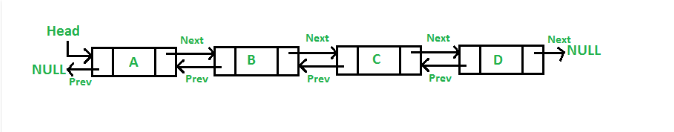
\includegraphics[width=12cm,height=6cm,keepaspectratio]{5.png}    
\end{figure}
\section{Task}  
\subsection{Procedure: Task 1 Implement DFS on graph}
Implement the DFS Depth First Search on the following graph:
\begin{figure}[H]
\centering
  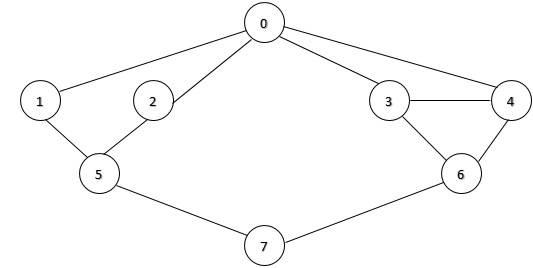
\includegraphics[width=12cm,height=6cm,keepaspectratio]{graph.png}    
\end{figure}
\begin{lstlisting}[language=C++]
#include<iostream>
#include<list>
using namespace std;

class Graph{
	int V;
	list<int> *adj;
	void DFSgraph(int v, bool visited[]){
		visited[v] = true;
		cout<< v << " ";
		
		list<int>::iterator i;
	    for (i = adj[v].begin(); i != adj[v].end(); i++)
	    	if (!visited[*i])
	    		DFSgraph(*i, visited);
	}
	public:
		Graph(int V){
			this->V = V;
			adj = new list<int>[V];
		}
		
		void addEdge(int u, int v){
			adj[u].push_back(v);
			adj[v].push_back(u);
		}
		
		void printGraph(){
			list<int>::iterator v;
			for(int i=0; i<V; i++){
		cout << "\n Adjacency list of vertex "<< i << "\n head ";
			for(v = adj[i].begin(); v != adj[i].end(); v++){
					cout << " -> " << *v;
				}
				cout<<"\n";
			}
			cout<<"\n\n";
		}
		
		void DFS(int root){
			bool visited[V];
			for (int i = 0; i < V; i++)
		        visited[i] = false;
		        
		    DFSgraph(root, visited);
		}
};

int main(){
	Graph graph1(8);
	graph1.addEdge(0, 1);
	graph1.addEdge(0, 2);
	graph1.addEdge(0, 3);
	graph1.addEdge(0, 4);
	graph1.addEdge(1, 5);
	graph1.addEdge(2, 5);
	graph1.addEdge(3, 4);
	graph1.addEdge(3, 6);
	graph1.addEdge(4, 6);
	graph1.addEdge(5, 7);
	graph1.addEdge(6, 7);
	graph1.printGraph();
	cout << "Following is Depth First Traversal of the above 
graph (starting from vertex 0) \n\n";
	graph1.DFS(0);
	return 0;
}
\end{lstlisting}
 \textbf Output: Consider the Figure 1 for the output of the above code in the end of this document.

\textbf{Source Code} \\
https://goo.gl/ccBvqK

\begin{figure}[b!]
\centering
  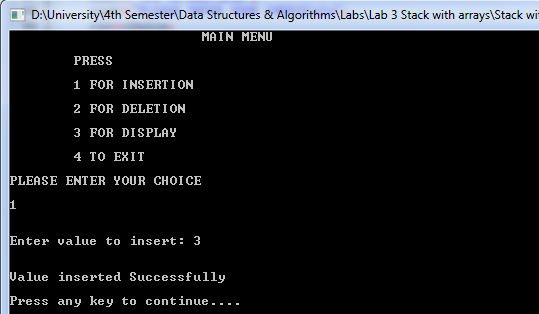
\includegraphics[width=12cm,height=6cm,keepaspectratio]{1.png}
\caption{Depth First Search implementation on graph}
\label{Figure:1}    
\end{figure}

\section{Conclusion}
\justify Graphs are used to represent many real life applications: Graphs are used to represent networks. The networks may include paths in a city or telephone network or circuit network. Depth First Search algorithm can be implemented on graphs to visit every node in the shortest path, graphs may contain cycles, so we may come to the same node again. To avoid processing a node more than once, we use a boolean visited array.\\~\\

\tab[6cm] \noindent\rule{6cm}{0.4pt}\\
\tab[6cm] (Concerned Teacher/Lab Engineer)


 
\end{document}                          % The required last line
